
\documentclass[journal]{IEEEtran}
\usepackage[utf8]{inputenc}
\usepackage{graphicx}
\usepackage{subfig}
\usepackage{amsmath}
\usepackage{amsthm}
\usepackage{multicol}
\usepackage{ragged2e}
\usepackage{siunitx}
\usepackage{tikz}
\usepackage{tikz-3dplot}
\usetikzlibrary{shapes,arrows}
\usepackage{pgfplots}
\pgfplotsset{compat=newest}
\pgfplotsset{plot coordinates/math parser=false}
\newlength\figureheight
\newlength\figurewidth
\renewcommand\labelitemi{--}
\newtheorem*{remark}{Remark}

\usepackage{ifthen}
\usepackage{ifpdf}
\ifpdf
\usepackage[pdftex]{hyperref}
\else
\usepackage{hyperref}
\fi
\usepackage{color}


\begin{document}

\title{Space Exploration Engineering\\
Mid-term Report A1}

\author{Romain~Pessia — Student Number 81723435 \\
Fall 2017, Keio University }%

\maketitle

\section*{Introduction}

In this short study, we will look into two methods for orbit transfer---namely, the \textit{Hohmann transfer} and the \textit{bi-elliptic transfer}. In particular, our goal is to compare the energy efficiency of both methods for different configurations of the initial and final orbit.

\section*{Energy efficiency for an orbit transfer}

To compare both transfers, we need to define a variable to assess energy efficiency identically for both methods. To that effect, we use a dimensionless metric---the relative speed variation between the two orbits---which will be different for the Hohmann transfer and the bi-elliptic transfer. Using the same notation as the problem statement, the calculation of this metric goes as follows for the Hohmann transfer:

\begin{equation}
    \Delta v = \left|\Delta v_1 \right| + \left|\Delta v_2 \right|
\end{equation}
\begin{equation}
    \Delta v_1 = \sqrt{\frac{\mu}{r_1}}\left( \sqrt{\frac{2r_2}{r_1+r_2}} -1 \right)
\end{equation}
\begin{equation}
    \Delta v_2 = \sqrt{\frac{\mu}{r_2}}\left( 1- \sqrt{\frac{2r_1}{r_1+r_2}} \right)
\end{equation}

with $\Delta v$ the overall speed difference between the two orbits, $\Delta v_1$ the speed difference upon entering the elliptic orbit from the circular orbit at $r=r_1$, and $\Delta v_2$ the speed difference upon leaving the elliptic orbit for the circular orbit at $r=r_2$.

For the bi-elliptic transfer, the following formulae apply:

\begin{equation}
    \Delta v  = \left|\Delta v_1 \right| + \left| \Delta v_2 \right| + \left| \Delta v_3 \right|
\end{equation}
\begin{equation}
    \Delta v_1 = \sqrt{\frac{2\mu}{r_1}-\frac{\mu}{a_1}}-\frac{\mu}{r_1}
\end{equation}
\begin{equation}
    \Delta v_2 = \sqrt{\frac{2\mu}{r_m}-\frac{\mu}{a_2}} - \sqrt{\frac{2\mu}{r_m}-\frac{\mu}{a_1}}
\end{equation}
\begin{equation}
    \Delta v_3 = \sqrt{\frac{2\mu}{r_2}-\frac{\mu}{a_2}}-\frac{\mu}{r_2}
\end{equation}

where $a_1$ and $a_2$ are the semimajor axes of the two elliptic transfer orbits, and $r_m$ is the transfer radius between the two elliptic orbits.

We can thus define the dimensionless speed variation of the transfer as

\begin{equation}
    \Delta \bar{v} = \frac{\Delta v}{v_0}
\end{equation}

where $v_0$ is in both cases $\sqrt{\frac{\mu}{r_1}}$.

\section*{Computer simulation and result analysis}

We developed a C++ program\cite{git_program} that calculates the energy efficiency of both transfer methods based on a certain value of $r_{21}$. For the bi-elliptical transfer, there is an additional free parameter, which we control \textit{via} the ratio $r_{m1}$.

We can thus draw the evolution of the relative speed variation between the initial and final orbits ($\Delta \bar{v}$, which is a classic feature to study when comparing the two methods. The plot in question can be found in Figure \ref{plot:vbar}.


\begin{figure}[htp!]
  \centering
  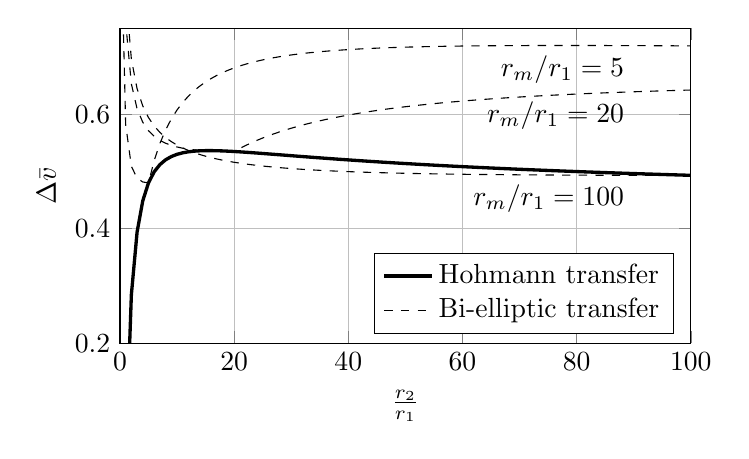
\begin{tikzpicture}

\begin{axis}[%
view={0}{90},
width=7.25cm,
height=4cm,
scale only axis,
xmin=0, xmax=100,
xlabel={$\frac{r_2}{r_1}$},
xmajorgrids,
ymin=0.2, ymax=0.75,
ymajorgrids,
ylabel={$\Delta \bar{v}$},
legend cell align=left,
legend pos = south east,
legend style={align=left}]
\addplot [
color=black,
very thick,
mark=none,
mark options={solid}
]
coordinates{
(1,0)(2,0.284457)(3,0.393847)(4,0.448683)(5,0.480009)(6,0.499338)(7,0.511858)(8,0.52022)(9,0.525903)(10,0.529788)(11,0.532426)(12,0.53418)(13,0.535292)(14,0.535931)(15,0.536218)(16,0.536239)(17,0.536059)(18,0.535725)(19,0.535273)(20,0.534731)(21,0.534121)(22,0.533459)(23,0.532759)(24,0.53203)(25,0.53128)(26,0.530517)(27,0.529746)(28,0.52897)(29,0.528193)(30,0.527417)(31,0.526645)(32,0.525879)(33,0.525119)(34,0.524367)(35,0.523623)(36,0.522889)(37,0.522165)(38,0.52145)(39,0.520746)(40,0.520053)(41,0.51937)(42,0.518698)(43,0.518036)(44,0.517385)(45,0.516745)(46,0.516115)(47,0.515495)(48,0.514885)(49,0.514286)(50,0.513696)(51,0.513116)(52,0.512545)(53,0.511983)(54,0.511431)(55,0.510887)(56,0.510353)(57,0.509826)(58,0.509308)(59,0.508799)(60,0.508297)(61,0.507803)(62,0.507317)(63,0.506838)(64,0.506366)(65,0.505902)(66,0.505445)(67,0.504994)(68,0.50455)(69,0.504113)(70,0.503682)(71,0.503257)(72,0.502838)(73,0.502425)(74,0.502018)(75,0.501617)(76,0.501221)(77,0.500831)(78,0.500446)(79,0.500067)(80,0.499692)(81,0.499322)(82,0.498958)(83,0.498598)(84,0.498242)(85,0.497892)(86,0.497546)(87,0.497204)(88,0.496866)(89,0.496533)(90,0.496204)(91,0.495879)(92,0.495558)(93,0.495241)(94,0.494927)(95,0.494618)(96,0.494312)(97,0.494009)(98,0.493711)(99,0.493415)(100,0.493123)

};
\addlegendentry{Hohmann transfer};

\addplot [
color=black,
dashed,
mark=none,
mark options={solid}
]
coordinates{(0,1)(1,0.581989)(2,0.508905)(3,0.488241)(4,0.481479)(5,0.480009)(6,0.518894)(7,0.548773)(8,0.572401)(9,0.591503)(10,0.607222)(11,0.620346)(12,0.631436)(13,0.640905)(14,0.649062)(15,0.656143)(16,0.662332)(17,0.667773)(18,0.672583)(19,0.676856)(20,0.680666)(21,0.684079)(22,0.687146)(23,0.68991)(24,0.69241)(25,0.694676)(26,0.696735)(27,0.69861)(28,0.700322)(29,0.701887)(30,0.70332)(31,0.704634)(32,0.705842)(33,0.706953)(34,0.707976)(35,0.708919)(36,0.709789)(37,0.710593)(38,0.711336)(39,0.712023)(40,0.712659)(41,0.713247)(42,0.713793)(43,0.714298)(44,0.714766)(45,0.7152)(46,0.715602)(47,0.715975)(48,0.716321)(49,0.716641)(50,0.716937)(51,0.717212)(52,0.717466)(53,0.7177)(54,0.717917)(55,0.718117)(56,0.718302)(57,0.718472)(58,0.718628)(59,0.718771)(60,0.718902)(61,0.719021)(62,0.71913)(63,0.719229)(64,0.719318)(65,0.719399)(66,0.719471)(67,0.719535)(68,0.719592)(69,0.719642)(70,0.719685)(71,0.719722)(72,0.719753)(73,0.719778)(74,0.719798)(75,0.719813)(76,0.719824)(77,0.719829)(78,0.719831)(79,0.719829)(80,0.719823)(81,0.719813)(82,0.7198)(83,0.719784)(84,0.719764)(85,0.719742)(86,0.719717)(87,0.719689)(88,0.719659)(89,0.719627)(90,0.719593)(91,0.719556)(92,0.719517)(93,0.719477)(94,0.719434)(95,0.719391)(96,0.719345)(97,0.719298)(98,0.719249)(99,0.719199)(100,0.719148)
}
node [pos=0.9, below left]{$r_m/r_1=5$};
\addlegendentry{Bi-elliptic transfer};

\addplot [
color=black,
dashed,
mark=none,
mark options={solid}
]
coordinates{(0,1)(1,0.760262)(2,0.652827)(3,0.609369)(4,0.585721)(5,0.571018)(6,0.561157)(7,0.554219)(8,0.549179)(9,0.545437)(10,0.542619)(11,0.540479)(12,0.538847)(13,0.537606)(14,0.536669)(15,0.535972)(16,0.535466)(17,0.535116)(18,0.534891)(19,0.534769)(20,0.534731)(21,0.540119)(22,0.545132)(23,0.549805)(24,0.554174)(25,0.558265)(26,0.562104)(27,0.565714)(28,0.569113)(29,0.57232)(30,0.575348)(31,0.578213)(32,0.580927)(33,0.583501)(34,0.585945)(35,0.588268)(36,0.590478)(37,0.592584)(38,0.594592)(39,0.596508)(40,0.598338)(41,0.600087)(42,0.601761)(43,0.603364)(44,0.6049)(45,0.606372)(46,0.607785)(47,0.609141)(48,0.610445)(49,0.611698)(50,0.612903)(51,0.614062)(52,0.615179)(53,0.616255)(54,0.617292)(55,0.618293)(56,0.619258)(57,0.620189)(58,0.621089)(59,0.621958)(60,0.622798)(61,0.62361)(62,0.624396)(63,0.625157)(64,0.625893)(65,0.626605)(66,0.627296)(67,0.627965)(68,0.628613)(69,0.629242)(70,0.629852)(71,0.630444)(72,0.631018)(73,0.631576)(74,0.632118)(75,0.632643)(76,0.633155)(77,0.633651)(78,0.634134)(79,0.634603)(80,0.63506)(81,0.635504)(82,0.635936)(83,0.636357)(84,0.636766)(85,0.637165)(86,0.637553)(87,0.637931)(88,0.6383)(89,0.638659)(90,0.639008)(91,0.639349)(92,0.639682)(93,0.640006)(94,0.640322)(95,0.640631)(96,0.640932)(97,0.641225)(98,0.641512)(99,0.641792)(100,0.642065)
}
node [pos=0.9, below left]{$r_m/r_1=20$};

\addplot [
color=black,
dashed,
mark=none,
mark options={solid}
]
coordinates{(0,1)(1,0.81439)(2,0.695967)(3,0.644426)(4,0.614233)(5,0.593984)(6,0.579293)(7,0.568073)(8,0.559185)(9,0.551951)(10,0.545937)(11,0.540854)(12,0.536497)(13,0.532722)(14,0.529418)(15,0.526502)(16,0.523912)(17,0.521596)(18,0.519514)(19,0.517633)(20,0.515927)(21,0.514373)(22,0.512953)(23,0.511651)(24,0.510454)(25,0.509351)(26,0.508332)(27,0.507388)(28,0.506512)(29,0.505699)(30,0.504941)(31,0.504234)(32,0.503575)(33,0.502958)(34,0.50238)(35,0.501838)(36,0.50133)(37,0.500853)(38,0.500404)(39,0.499982)(40,0.499584)(41,0.49921)(42,0.498856)(43,0.498523)(44,0.498208)(45,0.497911)(46,0.49763)(47,0.497365)(48,0.497113)(49,0.496876)(50,0.496651)(51,0.496438)(52,0.496236)(53,0.496045)(54,0.495865)(55,0.495693)(56,0.495531)(57,0.495378)(58,0.495232)(59,0.495094)(60,0.494964)(61,0.49484)(62,0.494723)(63,0.494613)(64,0.494508)(65,0.494409)(66,0.494315)(67,0.494227)(68,0.494143)(69,0.494064)(70,0.49399)(71,0.493919)(72,0.493853)(73,0.493791)(74,0.493733)(75,0.493678)(76,0.493626)(77,0.493578)(78,0.493533)(79,0.493491)(80,0.493452)(81,0.493415)(82,0.493382)(83,0.49335)(84,0.493321)(85,0.493295)(86,0.493271)(87,0.493249)(88,0.493229)(89,0.49321)(90,0.493194)(91,0.49318)(92,0.493167)(93,0.493157)(94,0.493147)(95,0.49314)(96,0.493134)(97,0.493129)(98,0.493126)(99,0.493124)(100,0.493123)
}
node [pos=0.9, below left]{$r_m/r_1=100$};

\end{axis}
\end{tikzpicture}%
  \caption{Speed variation of Hohmann and bi-elliptic transfers}
  \label{plot:vbar}
\end{figure}

As we can see, when speaking strictly in terms of normalized speed difference, the Hohmann transfer is more efficient than the bi-elliptic transfer for low values of $r_{21}$, no matter the value of $r_{m1}$. To find the limit value of $r_{21}$ above which the Hohmann transfer stops being always optimal, one can calculate the point of intersection between the speed variation curve for the Hohmann transfer and that of the bi-elliptic transfer for $r_{m1}=+\infty$, which gives the value $r_{{21}_{max}}\approx 11.94$.

Conversely, if we make the assumption that $r_m \geq r_2$, there is a minimal value of 
$r_{21}$ above which any value of $r_{m1}$ greater than $r_{21}$ corresponds to a bi-elliptic transfer more efficient than the Hohmann transfer. To find that value, one needs to calculate the smallest value of $r_{21}$ such that the normalized speed variation for any $r_{m1}\geq r_{21}$ is lower for the bi-elliptic transfer. That minimum value $r_{{21}_{min}}$ has a value of approximately 15.58.

\begin{remark}
We found those two particular values of $r_{21}$ by developing a short Matlab script which can be found in \cite{git_program}.
\end{remark}

For values of $r_{21}$ comprised between 11.94 and 15.58, whichever transfer is more efficient depends on the value of $r_{m1}$, as shown by Figure \ref{plot:vbar3}.

Figure \ref{plot:vbar2} shows a zoomed portion of Figure \ref{plot:vbar1}, showcasing the two limit values of $r_{21}$ mentioned earlier, and their graphical interpretation as the intersection of the energy efficiency curves. Figure \ref{plot:vbar3} illustrates the minimal value of $r_{m1}$ above which the bi-elliptic transfer is more efficient for values of $r_{21}$ between $11.94$ and $15.58$. Finally, Table \ref{table:1} shows in a condensed way which transfer is more efficient given the values of $r_{21}$ and $r_{m1}$.
\begin{table}[h!]
\centering
 \begin{tabular}{| c | c| c |} 
 \hline
 Value of $r_{21}$ & Value of $r_{m1}$ & Most efficient transfer \\
 \hline
 $r_{21} \leq 11.94$ & Any & Hohmann\\
 $11.94 < r_{21}  \leq 15.58$ & $r_{m1} > r_{m1_{min}}(r_{21}) $ &Hohmann\\
 $11.94 < r_{21}  \leq 15.58$ & $r_{m1} < r_{m1_{min}}(r_{21}) $ &Bi-elliptic\\
 $r_{21}> 15.58$ & $r_{m1} > r_{21}$ & Bi-elliptic\\
 \hline
\end{tabular}
\caption{Compared efficiency of Hohmann and bi-elliptic transfers}
\label{table:1}
\end{table}



\begin{figure}[htp!]
  \centering
  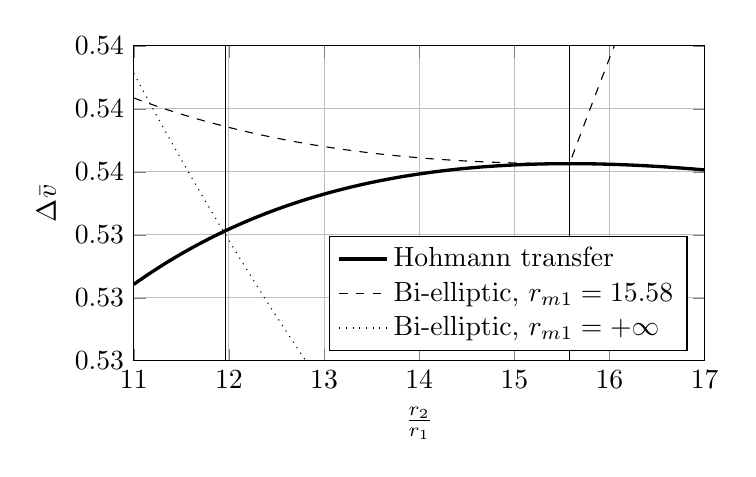
\begin{tikzpicture}

\begin{axis}[%
view={0}{90},
width=7.25cm,
height=4cm,
scale only axis,
xmin=11, xmax=17,
xlabel={$\frac{r_2}{r_1}$},
xmajorgrids,
ymin=0.530, ymax=0.540,
ymajorgrids,
ylabel={$\Delta \bar{v}$},
legend cell align=left,
legend pos = south east,
legend style={align=left}]
\addplot [
color=black,
very thick,
mark=none,
mark options={solid}
]
coordinates{
(11,0.532426)(11.0606,0.532555)(11.1212,0.53268)(11.1818,0.532803)(11.2424,0.532922)(11.303,0.533038)(11.3636,0.533152)(11.4242,0.533262)(11.4848,0.53337)(11.5455,0.533475)(11.6061,0.533577)(11.6667,0.533677)(11.7273,0.533774)(11.7879,0.533868)(11.8485,0.53396)(11.9091,0.53405)(11.9697,0.534137)(12.0303,0.534222)(12.0909,0.534304)(12.1515,0.534385)(12.2121,0.534463)(12.2727,0.534539)(12.3333,0.534612)(12.3939,0.534684)(12.4545,0.534753)(12.5152,0.534821)(12.5758,0.534886)(12.6364,0.53495)(12.697,0.535011)(12.7576,0.535071)(12.8182,0.535129)(12.8788,0.535185)(12.9394,0.535239)(13,0.535292)(13.0606,0.535343)(13.1212,0.535392)(13.1818,0.535439)(13.2424,0.535485)(13.303,0.535529)(13.3636,0.535572)(13.4242,0.535613)(13.4848,0.535653)(13.5455,0.535691)(13.6061,0.535727)(13.6667,0.535762)(13.7273,0.535796)(13.7879,0.535829)(13.8485,0.53586)(13.9091,0.535889)(13.9697,0.535918)(14.0303,0.535945)(14.0909,0.53597)(14.1515,0.535995)(14.2121,0.536018)(14.2727,0.53604)(14.3333,0.536061)(14.3939,0.536081)(14.4545,0.5361)(14.5152,0.536117)(14.5758,0.536133)(14.6364,0.536149)(14.697,0.536163)(14.7576,0.536176)(14.8182,0.536188)(14.8788,0.536199)(14.9394,0.536209)(15,0.536218)(15.0606,0.536226)(15.1212,0.536233)(15.1818,0.53624)(15.2424,0.536245)(15.303,0.536249)(15.3636,0.536253)(15.4242,0.536255)(15.4848,0.536257)(15.5455,0.536258)(15.6061,0.536258)(15.6667,0.536258)(15.7273,0.536256)(15.7879,0.536254)(15.8485,0.536251)(15.9091,0.536247)(15.9697,0.536242)(16.0303,0.536237)(16.0909,0.53623)(16.1515,0.536224)(16.2121,0.536216)(16.2727,0.536208)(16.3333,0.536199)(16.3939,0.536189)(16.4545,0.536179)(16.5152,0.536168)(16.5758,0.536157)(16.6364,0.536145)(16.697,0.536132)(16.7576,0.536118)(16.8182,0.536104)(16.8788,0.53609)(16.9394,0.536075)(17,0.536059)
};
\addlegendentry{Hohmann transfer};


\addplot [
color=black,
dashed,
mark=none,
mark options={solid}
]
coordinates{(11,0.538345)(11.0606,0.538277)(11.1212,0.538211)(11.1818,0.538146)(11.2424,0.538082)(11.303,0.538021)(11.3636,0.53796)(11.4242,0.537901)(11.4848,0.537844)(11.5455,0.537788)(11.6061,0.537733)(11.6667,0.537679)(11.7273,0.537627)(11.7879,0.537576)(11.8485,0.537527)(11.9091,0.537479)(11.9697,0.537431)(12.0303,0.537386)(12.0909,0.537341)(12.1515,0.537297)(12.2121,0.537255)(12.2727,0.537214)(12.3333,0.537174)(12.3939,0.537135)(12.4545,0.537097)(12.5152,0.53706)(12.5758,0.537024)(12.6364,0.536989)(12.697,0.536955)(12.7576,0.536923)(12.8182,0.536891)(12.8788,0.53686)(12.9394,0.53683)(13,0.536801)(13.0606,0.536773)(13.1212,0.536746)(13.1818,0.536719)(13.2424,0.536694)(13.303,0.536669)(13.3636,0.536645)(13.4242,0.536623)(13.4848,0.536601)(13.5455,0.536579)(13.6061,0.536559)(13.6667,0.536539)(13.7273,0.53652)(13.7879,0.536502)(13.8485,0.536485)(13.9091,0.536468)(13.9697,0.536452)(14.0303,0.536437)(14.0909,0.536422)(14.1515,0.536408)(14.2121,0.536395)(14.2727,0.536383)(14.3333,0.536371)(14.3939,0.53636)(14.4545,0.536349)(14.5152,0.536339)(14.5758,0.53633)(14.6364,0.536321)(14.697,0.536313)(14.7576,0.536306)(14.8182,0.536299)(14.8788,0.536292)(14.9394,0.536287)(15,0.536281)(15.0606,0.536277)(15.1212,0.536273)(15.1818,0.536269)(15.2424,0.536266)(15.303,0.536263)(15.3636,0.536261)(15.4242,0.53626)(15.4848,0.536259)(15.5455,0.536258)(15.6061,0.53647)(15.6667,0.53696)(15.7273,0.537447)(15.7879,0.537932)(15.8485,0.538413)(15.9091,0.538892)(15.9697,0.539368)(16.0303,0.539842)(16.0909,0.540313)(16.1515,0.540781)(16.2121,0.541246)(16.2727,0.541709)(16.3333,0.542169)(16.3939,0.542627)(16.4545,0.543082)(16.5152,0.543534)(16.5758,0.543984)(16.6364,0.544431)(16.697,0.544876)(16.7576,0.545319)(16.8182,0.545759)(16.8788,0.546197)(16.9394,0.546632)(17,0.547065)
};
\addlegendentry{Bi-elliptic, $r_{m1}=15.58$};

\addplot [
color=black,
dotted,
mark=none,
mark options={solid}
]
coordinates{(11,0.539126)(11.0606,0.538784)(11.1212,0.538445)(11.1818,0.538108)(11.2424,0.537775)(11.303,0.537444)(11.3636,0.537115)(11.4242,0.53679)(11.4848,0.536466)(11.5455,0.536146)(11.6061,0.535828)(11.6667,0.535512)(11.7273,0.535199)(11.7879,0.534888)(11.8485,0.53458)(11.9091,0.534274)(11.9697,0.53397)(12.0303,0.533669)(12.0909,0.53337)(12.1515,0.533073)(12.2121,0.532779)(12.2727,0.532486)(12.3333,0.532196)(12.3939,0.531908)(12.4545,0.531622)(12.5152,0.531338)(12.5758,0.531056)(12.6364,0.530776)(12.697,0.530498)(12.7576,0.530222)(12.8182,0.529949)(12.8788,0.529677)(12.9394,0.529407)(13,0.529138)(13.0606,0.528872)(13.1212,0.528608)(13.1818,0.528345)(13.2424,0.528084)(13.303,0.527825)(13.3636,0.527568)(13.4242,0.527313)(13.4848,0.527059)(13.5455,0.526807)(13.6061,0.526557)(13.6667,0.526308)(13.7273,0.526061)(13.7879,0.525815)(13.8485,0.525572)(13.9091,0.525329)(13.9697,0.525089)(14.0303,0.52485)(14.0909,0.524612)(14.1515,0.524376)(14.2121,0.524142)(14.2727,0.523909)(14.3333,0.523677)(14.3939,0.523447)(14.4545,0.523219)(14.5152,0.522992)(14.5758,0.522766)(14.6364,0.522542)(14.697,0.522319)(14.7576,0.522097)(14.8182,0.521877)(14.8788,0.521658)(14.9394,0.521441)(15,0.521225)(15.0606,0.52101)(15.1212,0.520796)(15.1818,0.520584)(15.2424,0.520373)(15.303,0.520163)(15.3636,0.519955)(15.4242,0.519747)(15.4848,0.519541)(15.5455,0.519337)(15.6061,0.519133)(15.6667,0.51893)(15.7273,0.518729)(15.7879,0.518529)(15.8485,0.51833)(15.9091,0.518132)(15.9697,0.517935)(16.0303,0.51774)(16.0909,0.517545)(16.1515,0.517352)(16.2121,0.51716)(16.2727,0.516969)(16.3333,0.516778)(16.3939,0.516589)(16.4545,0.516401)(16.5152,0.516214)(16.5758,0.516028)(16.6364,0.515843)(16.697,0.515659)(16.7576,0.515476)(16.8182,0.515294)(16.8788,0.515113)(16.9394,0.514933)(17,0.514754)
};
\addlegendentry{Bi-elliptic, $r_{m1}=+\infty$};

\addplot [
color=black,
solid,
mark=none,
mark options={solid}
]
coordinates{(11.96,0.53)(11.96,0.54)};

\addplot [
color=black,
solid,
mark=none,
mark options={solid}
]
coordinates{(15.58,0.53)(15.58,0.54)};

\end{axis}
\end{tikzpicture}%
  \caption{Highlight of the two values of interest for $r_{21}$, represented by the solid vertical lines}
  \label{plot:vbar2}
\end{figure}

\begin{figure}[htp!]
  \centering
  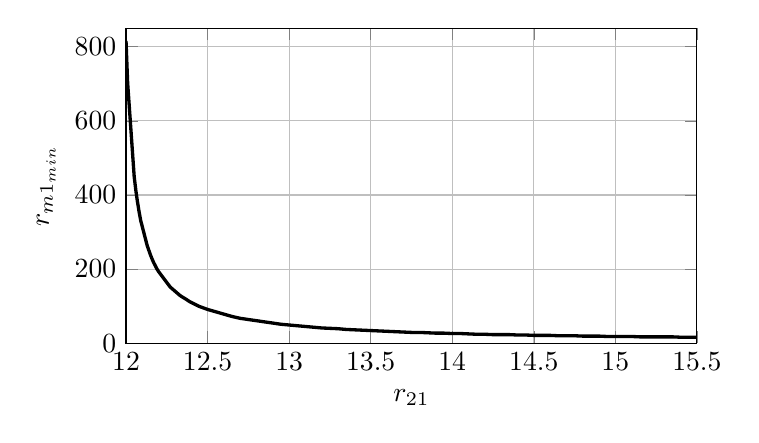
\begin{tikzpicture}

\begin{axis}[%
view={0}{90},
width=7.25cm,
height=4cm,
scale only axis,
xmin=12, xmax=15.5,
xlabel={$r_{21}$},
xmajorgrids,
ymin=0, ymax=850,
ymajorgrids,
ylabel={$r_{m1_{min}}$},
legend cell align=left,
legend pos = south east,
legend style={align=left}]
\addplot [
color=black,
very thick,
mark=none,
mark options={solid}
]
coordinates{
(12,816)
(1.201000e+01,702)
(1.205000e+01,450)
(1.206000e+01,413)
(1.207000e+01,382)
(1.208000e+01,355)
(1.209000e+01,331)
(1.213000e+01,263)
(1.215000e+01,238)
(1.216000e+01,227)
(1.217000e+01,217)
(1.219000e+01,200)
(1.220000e+01,193)
(1.220000e+01,193)
(1.227000e+01,152)
(1.228000e+01,148)
(1.233000e+01,129)
(1.234000e+01,126)
(1.237000e+01,118)
(1.238000e+01,115)
(1.239000e+01,112)
(1.245000e+01,99)
(1.250000e+01,91)
(1.265000e+01,72)
(1.270000e+01,67)
(1.295000e+01,51)
(13,49)
(1.315000e+01,43)
(1.320000e+01,41)
(1.325000e+01,40)
(1.330000e+01,39)
(1.335000e+01,37)
(1.340000e+01,36)
(1.345000e+01,35)
(1.350000e+01,34)
(1.355000e+01,33)
(1.360000e+01,32)
(1.365000e+01,31)
(1.370000e+01,30)
(1.375000e+01,29)
(1.380000e+01,29)
(1.385000e+01,28)
(1.390000e+01,27)
(1.395000e+01,27)
(14,26)
(1.405000e+01,26)
(1.410000e+01,25)
(1.415000e+01,24)
(1.420000e+01,24)
(1.425000e+01,23)
(1.430000e+01,23)
(1.435000e+01,23)
(1.440000e+01,22)
(1.445000e+01,22)
(1.450000e+01,21)
(1.455000e+01,21)
(1.460000e+01,21)
(1.465000e+01,20)
(1.470000e+01,20)
(1.475000e+01,20)
(1.480000e+01,19)
(1.485000e+01,19)
(1.490000e+01,19)
(1.495000e+01,18)
(15,18)
(1.505000e+01,18)
(1.510000e+01,18)
(1.515000e+01,17)
(1.520000e+01,17)
(1.525000e+01,17)
(1.530000e+01,17)
(1.535000e+01,17)
(1.540000e+01,16)
(1.545000e+01,16)
(1.550000e+01,16)
};

\end{axis}
\end{tikzpicture}%
  \caption{Minimum value of $r_{m1}$ above which the bi-elliptic transfer is more efficient than the Hohmann transfer}
  \label{plot:vbar3}
\end{figure}

\section*{Conclusion and open questions}

In this short study, we showed the relative efficiency of two classic orbit methods using a simple criterion based on normalized speed variation. This analysis, though limited, has however allowed us to clearly define in what situations either transfer is more efficient with regard to that criterion.

However, there are several factors that were unaccounted for, one of the most notable being the transfer time. Indeed, one of the notorious drawbacks of the bi-elliptic transfer over the Hohmann transfer is its long transfer time:

\begin{equation}
    t_{Hohmann}=\pi \sqrt{\frac{(r_1+r_2)^3}{2\mu}}
\end{equation}
\begin{equation}
    t_{Bi-elliptic} = \pi \sqrt{\frac{(r_1+r_m)^3}{2\mu}} + \pi \sqrt{\frac{(r_2+r_m)^3}{2 \mu}}
\end{equation}

Using the above formulae, a possible extension of this study would be to consider both a normalized speed criterion and a normalized time criterion. We could then, for each transfer method, look into the evolution of both criteria as a function of  $r_{21}$ and $r_{m1}$. In particular, for the bi-elliptic transfer, one possible approach would be to use (for a given value of $r_{21}$) a genetic algorithm in order to find the Pareto frontier from all the points of data obtained with different values of $r_{m1}$. Knowing the Pareto frontier for any value of $r_{21}$, we could then compare the multi-objective efficiency of both transfers depending on the relative weight associated with each criterion.

\appendices

\begin{thebibliography}{9}
\bibitem{git_program} 
Romain Pessia. 
\textit{Hohmann and bi-elliptical transfer energy efficiency}. 
Github project on \href{https://github.com/romainpessia/Hohmann-and-bi-elliptical-transfer-energy-efficiency}{https://github.com/romainpessia/Hohmann-and-bi-elliptical-transfer-energy-efficiency}, 2017.
\end{thebibliography}

\end{document}


